\documentclass{article}

\usepackage{arxiv}

\usepackage[utf8]{inputenc} % allow utf-8 input
\usepackage[T1]{fontenc}    % use 8-bit T1 fonts
\usepackage{lmodern}        % https://github.com/rstudio/rticles/issues/343
\usepackage{hyperref}       % hyperlinks
\usepackage{url}            % simple URL typesetting
\usepackage{booktabs}       % professional-quality tables
\usepackage{amsfonts}       % blackboard math symbols
\usepackage{nicefrac}       % compact symbols for 1/2, etc.
\usepackage{microtype}      % microtypography
\usepackage{graphicx}

\title{Madurez de la Industria 4.0 Transformación bajo los paradigmas de
la emergente Industria 5.0}

\author{
    Luis Patricio Torres Gómez
    \thanks{Los autores desean agradecer a Doctorado Interinstitucional
en Ingeniería Industrial sede Universidad Nacional de Cuyo}
   \\
    Facultad de Ingeniería UNCuyo \\
    Universidad Nacional de Cuyo \\
  Ciudad Universitaria CP 5502 Edificio de Ingeniería Mendoza
Argentina. \\
  \texttt{\href{mailto:patricio.torres@ucvp.edu.cl}{\nolinkurl{patricio.torres@ucvp.edu.cl}}} \\
   \And
    Lorena Bearzzotti
   \\
    Departamento de Ingeniería en Transporte \\
    Universidad Católica de Valparaíso \\
  Avenida Brasil 2147, esquina General Cruz, Edificio ICT, Valparaíso,
Chile \\
  \texttt{\href{mailto:lorena.bearzotti@pucv.cl}{\nolinkurl{lorena.bearzotti@pucv.cl}}} \\
  }


% tightlist command for lists without linebreak
\providecommand{\tightlist}{%
  \setlength{\itemsep}{0pt}\setlength{\parskip}{0pt}}

% From pandoc table feature
\usepackage{longtable,booktabs,array}
\usepackage{calc} % for calculating minipage widths
% Correct order of tables after \paragraph or \subparagraph
\usepackage{etoolbox}
\makeatletter
\patchcmd\longtable{\par}{\if@noskipsec\mbox{}\fi\par}{}{}
\makeatother
% Allow footnotes in longtable head/foot
\IfFileExists{footnotehyper.sty}{\usepackage{footnotehyper}}{\usepackage{footnote}}
\makesavenoteenv{longtable}

% Pandoc citation processing
%From Pandoc 3.1.8
% definitions for citeproc citations
\NewDocumentCommand\citeproctext{}{}
\NewDocumentCommand\citeproc{mm}{%
  \begingroup\def\citeproctext{#2}\cite{#1}\endgroup}
\makeatletter
 % allow citations to break across lines
 \let\@cite@ofmt\@firstofone
 % avoid brackets around text for \cite:
 \def\@biblabel#1{}
 \def\@cite#1#2{{#1\if@tempswa , #2\fi}}
\makeatother
\newlength{\cslhangindent}
\setlength{\cslhangindent}{1.5em}
\newlength{\csllabelwidth}
\setlength{\csllabelwidth}{3em}
\newenvironment{CSLReferences}[2] % #1 hanging-indent, #2 entry-spacing
 {\begin{list}{}{%
  \setlength{\itemindent}{0pt}
  \setlength{\leftmargin}{0pt}
  \setlength{\parsep}{0pt}
  % turn on hanging indent if param 1 is 1
  \ifodd #1
   \setlength{\leftmargin}{\cslhangindent}
   \setlength{\itemindent}{-1\cslhangindent}
  \fi
  % set entry spacing
  \setlength{\itemsep}{#2\baselineskip}}}
 {\end{list}}
\usepackage{calc}
\newcommand{\CSLBlock}[1]{#1\hfill\break}
\newcommand{\CSLLeftMargin}[1]{\parbox[t]{\csllabelwidth}{#1}}
\newcommand{\CSLRightInline}[1]{\parbox[t]{\linewidth - \csllabelwidth}{#1}\break}
\newcommand{\CSLIndent}[1]{\hspace{\cslhangindent}#1}

\begin{document}
\maketitle


\begin{abstract}
After almost a decade of Industry 4.0 emergence, which is marked by the
total automation of manufacturing and the creation of intelligent
self-control networks throughout the value chain (Yañez, 2017), what the
European Commission calls Industry 5.0 emerges, which, unlike the
previous one, is based on the creation of value (Xu et al., 2021) and
the achievement of social and ecological objectives with a holistic,
sustainable and human-centered approach (Hein-Pensel et al., 2023),
breaking down the barriers of efficiency and productivity, towards a
higher appreciation of respect for human values and the contribution to
the vital needs of society, towards an industry centered on the human
being, sustainable and resilient (Golovianko et al., 2023). The path
that organizations must take towards the application of the I5.0
paradigms necessarily requires the application of the enabling
technologies of I4.0, but in a productive symbiosis with the basic
pillars of I5.0, that is, the virtuous triad of the human-centric
approach, resilience and sustainability at the level of its
comprehensive management as a way of guaranteeing business continuity.
In order to enable the concepts of I5.0 at the level of company
management, it is essential to know the initial state in which they are,
in order to project a binding potential development strategy from there.
In this sense, maturity models have been a useful tool for decades for
determining and qualifying the capabilities of elements that mature and,
as a consequence of their application, allow the determination of
appropriate actions to reach a higher level of maturity (Kohlegger et
al., 2009) and, from the perspective of Industry 5.0 and its connection
with 4.0 technologies, it turns out to be a fundamental element. In this
context, the research presented has as its central objective, based on a
systematic review of the literature, to understand the reality regarding
the existing maturity models linked to I5.0 and the connection they have
with Industry 4.0 and its enabling technologies.
\end{abstract}

\keywords{
    Industry 5.0
   \and
    Productive innovation
   \and
    Industrial Maturity model.
  }

\section{Introduccion}\label{introduccion}

La industria enfrenta hoy la llamada Revolución Industrial 4.0, marcada
por la automatización total de la manufactura y la creación de redes
inteligentes de autocontrol en toda la cadena de valor (Yáñez, 2017), lo
cual exigirá a la industria transformaciones profundas basadas en
principios fundamentales como la interoperatibilidad, descentralización,
capacidad en tiempo real, virtualización y modularización, las que
permitirán la autorregulación y la integración digital dentro y fuera de
los límites de la organización (Galar et al., 2020, Prause, 2019). Esta
transformación de la gestión de negocios, será conducida a través de
redes productivas globales (maquinaria, sistemas de almacenamiento e
instalaciones de producción) en forma de Sistemas Ciber Físicos (CPS)
que intercambiarán información autónomamente, ejecutando procesos y
acciones de control independientes en tres dimensiones: la cadena de
valor, el ciclo de vida del producto y la integración de los sistemas de
fabricación en red (Galar et al., 2020), optimizando sus procesos,
mejorando la rentabilidad y en consecuencia, la continuidad y
sustentabilidad del negocio, en un proceso transformativo que requerirá
de habilitadores digitales, es decir, tecnologías digitales 4.0 o ``Key
Enabling Technologies'' (KETs) (Yáñez, 2017). Sin embargo, la irrupción
desarticulada de esta nueva revolución, al igual que en anteriores
revoluciones industriales, generará una brecha tecnológica entre países,
dada la disparidad en el desarrollo y apropiación de tecnología, debido
a limitaciones financieras, organizacionales y el contexto en el cual
las organizaciones se desenvuelven, situación homologable a las empresas
en función de su tamaño, derivado del surgimiento de fuerzas que limitan
y dificultan la adopción de tecnologías al interior de las Pequeñas y
Medianas Empresas (PyMEs), evidenciando una realidad dispar de la
gestión innovadora entre éstas y las grandes compañías (Reyes, 2018) y
cuyas causas pueden ser diversas y estar relacionadas con factores como
la escasez de recursos financieros, el acceso no igualitario a
financiamiento, la falta de tecnología, por desconocimiento o limitación
de recursos, la capacitación del personal e inmadurez del soporte TI,
resistencia al cambio, una falta de claridad en los beneficios de la
implementación, el riesgo en la seguridad de los datos y en los puestos
de trabajo, la falta de cultura digital interna, el reducido tamaño de
la empresa, la falta de visión digital y liderazgo de la alta dirección
para asumir el proceso de transformación 4.0, la ausencia o
insuficiencia de políticas públicas, que desde un estado activo, ayuden
a fortalecer las condiciones para su desarrollo, entre otras (Arnold et
al., 2018; Gatica y Ramos, 2022; Maggi et al.~2020; Mazzucato y
McPherson, 2019; Prause, 2019; Reyes, 2018; Wischmann et al.~2015,
citado por Prause, 2019). En tal sentido, para disminuir o al menos
poner freno a estas brechas emergentes, se requiere de un actuar con
convicción, determinación y liderazgo en el desarrollo de una estrategia
para la implementación exitosa de la Industria 4.0 (I4.0) y como
consecuencia de ello, alcanzar los beneficios y el mejoramiento esperado
de la introducción de sus tecnologías habilitantes, en un proceso que
debe moverse dentro de un marco referencial que permita visualizar las
tecnologías de soporte físicas y digitales capaces de apoyar los
procesos de la cadena de suministro global desde el abastecimiento hasta
el mercado, pasando por la producción y la distribución de los productos
y/o servicios de la empresa, considerando las características propias de
la cadena de suministro en la que se inserta una industria en particular
y los resultados estratégicos esperados en el ámbito de la I4.0 (He y
Turner, 2021). En este camino, resulta clave conocer el nivel de
desarrollo tecnológico en que se encuentra la industria, cualquiera sea
su naturaleza y el sector económico al cual pertenezca y para ello, los
modelos de madurez (MMs) constituyen una herramienta útil para la
determinación y calificación de las capacidades de los elementos que
maduran y como consecuencia de su aplicación, permitir la determinación
de acciones apropiadas para alcanzar un nivel más alto de madurez
(Kohlegger et al., 2009), en un proceso de mejoramiento continuo, que en
el contexto de la I4.0, contribuirá a determinar el estado de
preparación o el nivel de madurez en el uso de las tecnologías
habilitantes asociadas y proporcionar medidas para mejorar su status
tecnológico (Kieroth et al., 2022), coaccionando patrones predecibles de
evolución y cambio organizacional, que representan teorías de evolución
y transformación de las capacidades de una organización a lo largo de un
camino definido, deseado o lógico, desde un estado inicial a maduro; y
en el que su nivel de madurez, se debe entender como la evidencia
objetiva de la capacidad respecto a una clase concreta de objetos y
dominio de aplicación. (Pöppelbuss y Röglinger, 2011, Röglinger et al.,
2012). De acuerdo a lo descrito por Pöppelbus y Röglinger, 2011, se
distinguen tres propósitos específicos de aplicación para el uso de los
MMs:

\begin{itemize}
\tightlist
\item
  Descriptivo: Modelos diseñados para la determinación del estado de
  situación actual.
\item
  Prescriptivo: Modelos normativos que proveen recomendaciones claras
  para la acción y guías para el desarrollo.
\item
  Comparativo: Modelos que permiten a las empresas y organizaciones ser
  localizadas y comparadas tanto interna como externamente.
\end{itemize}

Jacquez-Hernández y López (2018) señalan la existencia de muchos MMs
hacia la I4.0, pero que todos divergen en su metodología y criterios de
evaluación, concluyendo que no existe un modelo único y probado que
represente a todas las industrias y países, más aún si se considera la
novedad de la I4.0. Desde el punto de vista de la Industria 4.0, los MMs
pueden estar enfocados en objetos y dominios diversos que expliquen el
estado en que se encuentra la industria respecto de elementos y/o
factores establecidos en el objetivo central de dicha determinación.
Como, por ejemplo, MMs para determinar el nivel de preparación de la
industria hacia la implementación de la I4.0 o para mejorar dicho
proceso, para determinar la madurez respecto de la habilitación del
Internet de las Cosas (IoT) o el nivel de madurez de la I4.0 desde la
óptica de la cadena de suministro global, entre otras (de Carolis et
al., 2017¸ Jæger y Halse, 2017; Gracel \& Lebkowsky, 2017; Yañez, 2017;
Spaltini et al., 2022; Santos y Martinho, 2019; Rauch et al., 2020;
García-Reyes et al., 2022; Simetinger y Basl, 2022; Dahl, 2021) y por lo
tanto, la representación de la madurez bajo los paradigmas de la I4.0
estará condicionada por la dimensión que se defina como el objetivo
central del MM aplicado. A más de una década de la introducción de la
Industria 4.0, enfocada principalmente en el logro de los objetivos
económicos a través de la transformación digital y la automatización de
procesos de trabajo rutinarios (Hein-Pensel et al., 2023), la Comisión
Europea anunció el advenimiento de lo que llama la Industria 5.0, que a
diferencia de la anterior, impulsada por la habilitación de tecnologías,
se basa en la creación de valor (Xu et al, 2021) y el logro de objetivos
sociales y ecológicos basados en un enfoque holístico, sustentable y
centrado en el humano (Hein-Pensel et al., 2023), traspasando las vallas
de la eficiencia y la productividad, hacia una valorización superior de
respeto a los valores humanos y la contribución a las necesidades
vitales de la sociedad, poniendo el bienestar de los trabajadores junto
con otros valores humanos (relacionados con los empleados, los clientes
y la sociedad en general) en el centro de los procesos de
fabricación/producción, además de la ecología del planeta como factor
limitante y condicionante de la gestión productiva, como parte de un
proceso de transición hacia una industria centrada en el ser humano,
sostenible y resiliente (Golovianko et al, 2023). Según la Comisión
Europea (2021), ``La Industria 5.0 reconoce el poder de la industria
para alcanzar objetivos sociales más allá del empleo y el crecimiento,
para convertirse en un proveedor resistente de prosperidad, haciendo que
la producción respete los límites de nuestro planeta y situando el
bienestar del trabajador de la industria en el centro del proceso de
producción''. Sin embargo, la coexistencia de dos revoluciones
industriales plantea desafíos y preguntas que exigen discusiones y
aclaraciones relevantes como, por ejemplo, ¿Hasta qué punto la Industria
4.0 está centrada en la tecnología y olvida la centralidad humana, la
sustentabilidad y la resiliencia?; ¿Pueden las tecnologías habilitadoras
de la Industria 4.0 ayudar también a alcanzar los objetivos de la
Industria 5.0, o necesitamos desarrollar nuevas tecnologías de la
Industria 5.0?; ¿Es la Industria 5.0 una continuación cronológica de la
Industria 4.0, similar a sus predecesoras (desde la Industria 1.0 hasta
la Industria 4.0)?; ¿Vivimos entre dos revoluciones industriales o, en
realidad, una: la revolución tecnosocial?; ¿Cómo sería el proceso de
transformación de la industria hacia la Industria 4.0 y la Industria
5.0? (Xu et al, 2021). Sin perjuicio de la importancia de estas
preguntas y sus respectivas respuestas, lo que parece relevante en esta
dinámica vinculante de ambas industrias, es la necesidad de visualizar
de qué manera la industria y en especial las empresas del segmento PyMEs
se preparan, sobre la base de su realidad inherente, para la
incorporación de tecnologías habilitadoras consistentes con la Industria
4.0, pero que tomen en consideración los nuevos paradigmas que introduce
la naciente Industria 5.0, la que de alguna manera se hace cargo de la
mayor conciencia por la protección del medio ambiente, que en el mundo
de hoy se ha visto entre las organizaciones contemporáneas, las cuales
intentan establecerse como industrias sustentables, en un tránsito
``verde'', cuya definición incorpora diferentes aspectos ambientales
(Hasan et al., 2024). Es en este contexto de cambios paradigmáticos de
la Industria 4.0, que la complejidad de la digitalización se ve
incrementada debido a la incorporación de las nuevas dimensiones que
introduce la Industria 5.0, más aún si se considera el estrechamiento
colaborativo directo entre humanos y máquinas y en especial en el
segmento empresarial de las PyMEs, las que se ven enfrentadas a desafíos
mayores producto de la limitación de recursos para implementar una
estrategia de digitalización exitosa (Hein-Peinsel et al., 2023). Este
escenario confiere a los modelos de madurez (MMs) una valiosa relevancia
como herramienta para dar forma a la transición de la digitalización de
las empresas estratégicamente alineada, los cuales desde una perspectiva
integrada y holística, deberían llevar a la concepción de MMs de la
Industria 4.0 que contemplen los elementos claves de las dimensiones
específicas de la Industria 5.0 como la centralidad en el humano, la
resiliencia y la sustentabilidad y permitir una evaluación integral del
estado de preparación de las compañías hacia la implementación de
tecnologías y procesos disruptivos vinculados con la I4.0 (Hein-Pensel
et al., 2023). De acuerdo a la situación que se plantea, y en una
primera fase de investigación, se considera de interés conocer la
existencia de MMs de la I5.0 a nivel de la literatura y ver de qué forma
esos modelos se vinculan o se podrían vincular con los objetivos
particulares de la I4.0, generando una base de criterios y conceptos
integrados que permitan trabajar en la definición de un MM integrado
capaz de determinar el estado de madurez de las empresas desde la óptica
de la I4.0, pero teniendo en cuenta los elementos propios de la naciente
Industria 5.0.

\section{Justificación}\label{justificaciuxf3n}

La importancia de un enfoque centrado en el ser humano para todos los
aspectos de la digitalización cambia la forma de considerar los
requisitos de preparación para alcanzar ciertos niveles de madurez
digital y capacidad de implementación de las tecnologías habilitantes
que la sustentan. Esto significa que los MM deben ser una conjunción de
los MM de la Industria 4.0 y los tres pilares de la Industria 5.0, al
determinar la madurez digital (diseño centrado en el ser humano,
resiliencia y sustentabilidad), más aún si consideramos la estrecha
relación entre ambas industrias y la carencia de MM específicamente
desarrollados para la Industria 5.0 (Hein -- Pensel et al., 2022). La
implementación de la Industria 5.0 requiere un enfoque basado en la
integración de tecnologías avanzadas, como la inteligencia artificial,
la robótica, la computación de borde, entre otras, en un entorno de
fabricación centrado en el ser humano y la sustentabilidad, lo cual
implica el desarrollo de habilidades y conocimientos necesarios dentro
de las organizaciones para colaborar con estas tecnologías, así como
crear procesos de fabricación flexibles que puedan adaptarse a las
cambiantes demandas del mercado y a los impactos medioambientales
(Bajic, et al., 2023). La Industria 5.0 adquiere relevancia no sólo
debido a su objetivo de optimización de la producción y la eficiencia,
sino que también por poner el acento en el bienestar humano, la
sustentabilidad y la resiliencia, lo que permite preparar a las empresas
para enfrentar los desafíos del futuro (Arta et al., 2024),
evidenciándose en ella una singularidad tecnológica, que algunos como
Mantilla (2019), citado por Travez y Villafuerte (2023), la consideran
como una evolución dada por la personalización, la armonía de la
computación cognitiva e industrial (robots colaborativos), vinculando
los conceptos de Sociedad 5.0 e Industria 5.0 en el sentido de que ambos
se refieren a un cambio fundamental de nuestra sociedad y economía hacia
un nuevo paradigma, en una clara transformación de las industrias desde
las basadas en la producción a las basadas en el valor, centrándose en
los beneficios sociales y ambientales, así como en la obtención de
beneficios económicos, pero dando mayor énfasis al valor ambiental y
social, lo cual permitirá a las empresas asumir los desafíos de la
industria moderna y garantizar la sustentabilidad y continuidad del
negocio (European Commission, 2021). Es en este contexto de
trasformación de la industria, de constante cambio y evolución de los
factores internos y externos del entorno, exacerbado por la
globalización, que los paradigmas de la I4.0 y la I5.0 se conectan y
vinculan, haciéndose cargo de esta realidad con el propósito de, a nivel
de las organizaciones, lograr un fortalecimiento de su gestión
innovadora, incorporando tecnología con el objetivo de maximizar la
rentabilidad del negocio, pero con especial énfasis en una gestión
centrada en las personas, en la sustentabilidad y que en base al
monitoreo permanente de los factores del entorno cambiante y una actitud
resiliente, transformando riesgos en oportunidades, les permita dar
continuidad al negocio y conducirlas a posiciones de mayor relevancia en
el mercado. Claro es el panorama que enfrenta la industria, y este
desafío transformador implica llevar adelante procesos de adopción
tecnológica realistas, es decir, basados en las fortalezas y debilidades
de la empresa, particularmente en las PyMEs, con especial preocupación
en la internalización de los pilares de la I5.0. El punto de partida
entonces será conocer el nivel de madurez en que la empresa se encuentra
respecto a su preparación para enfrentar este reto y desde allí,
formular una estrategia de desarrollo realista capaz de conducirla a
estados de madurez superiores. Por tal razón, resulta de interés revisar
a nivel de la literatura la existencia de modelos de madurez tecnológica
5.0 y desde esa base, sentar las bases de investigaciones futuras
tendientes a medir el nivel de preparación de las empresas respecto a
los paradigmas de la I5.0 que les permitan modelar estrategias de
desarrollo potencial empresarial hacia niveles de posicionamiento
superior, con especial foco en las acciones que en tal sentido deben
emprender las empresas del segmento PyMEs, las cuales se ven fuertemente
expuestas a factores inhabilitantes y restrictivos que frenan o impiden
los procesos de adopción tecnológica.

\section{Objetivos}\label{objetivos}

\subsection{Objetivo general}\label{objetivo-general}

El objetivo general de la investigación es conocer a nivel de la
literatura la existencia de MMs basados en la Industria 5.0 y analizar
de qué manera estos se vinculan con los objetivos propios de la
Industria 4.0 hacia la definición de un modelo de madurez integrado.

\subsection{Objetivos específicos}\label{objetivos-especuxedficos}

\begin{itemize}
\item
  Analizar modelos existentes de la I5.0 desde la base de sus
  dimensiones y factores claves de su estructura y los niveles o
  estadios de madurez de evaluación.
\item
  Analizar y determinar los vínculos tecnológicos y relacionales de los
  MM de la I5.0 y sus pilares de sustentación, con aquellos propios de
  la Industria 4.0, como base para el desarrollo de investigaciones
  futuras que tengan como objetivo la proposición de un MM integrado
  I4.0 - I5.0.
\end{itemize}

\section{Materiales y Métodos}\label{materiales-y-muxe9todos}

El trabajo que se presenta consiste en una revisión sistemática de la
literatura (RSL) haciendo uso de las plataformas abiertas ``Dimensions
AI'' y ``Google Scholar'' y de la aplicación VOS Viewer y Excel para el
análisis y presentación de los resultados. El desarrollo de la
metodología de revisión bibliográfica fue conducido en base a un enfoque
estructurado por vom Brocke et al., 2009 y citado por Hein-Pensel et
al., 2022, el cual consta de tres fases y cinco etapas, según se muestra
en la Fig. 1.

\subsection{Generalidades}\label{generalidades}

El trabajo que se presenta consiste en una revisión sistemática de la
literatura (RSL) haciendo uso de las plataformas abiertas ``Dimensions
AI'' y ``Google Scholar'' y de la aplicación VOS Viewer y Excel para el
análisis y presentación de los resultados.

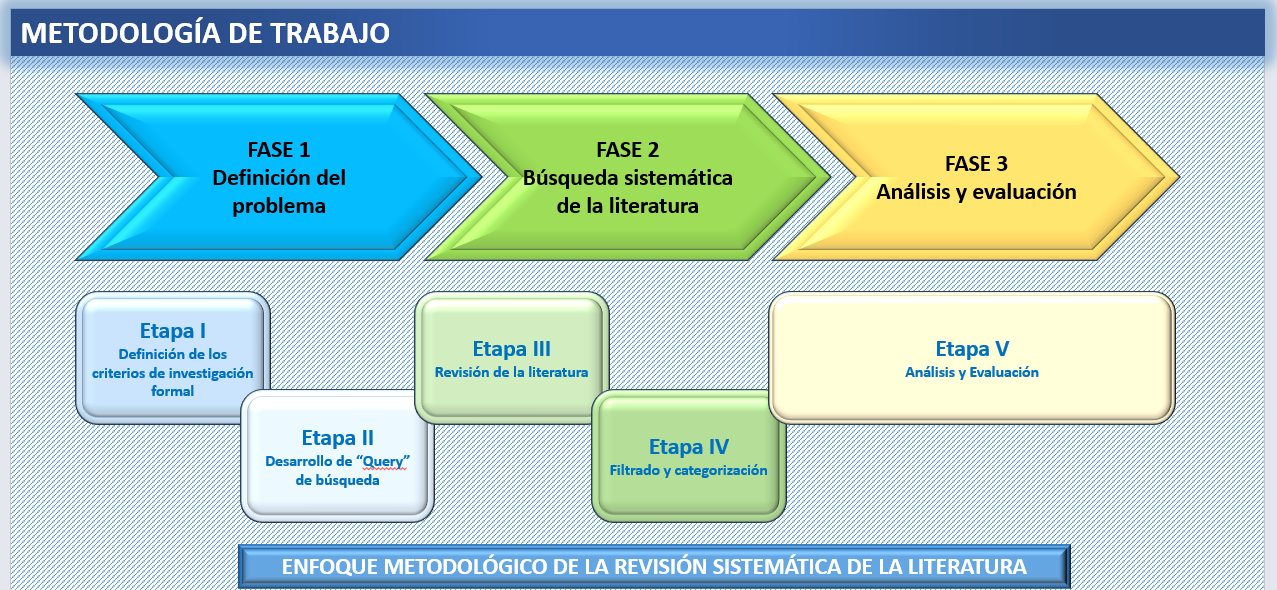
\includegraphics{images/clipboard-1820455245.png}

A modo de abundamiento y desde el punto de vista práctico, la conducción
metodológica se basó en la secuencia de actividades que se presentan a
continuación (Fig. 2):

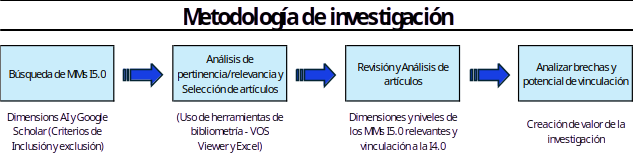
\includegraphics{images/clipboard-1289737579.png}

La RSL tuvo como punto de partida la búsqueda de investigaciones
relacionadas con la Industria 5.0, pero especialmente de aquellas
vinculadas con la presentación de modelos de madurez para medir el nivel
de preparación de las organizaciones para su implementación o de
criterios relevantes para su formulación.

Como complemento a esta base, se realizó una revisión de los artículos
del registro bibliográfico del autor.

Posterior a la obtención de la base general de artículos, se efectuó un
análisis de pertinencia/relevancia de los documentos encontrados, para
llegar finalmente a definir la base de revisión y análisis.

Como etapa final y como consecuencia de la obtención de la base de
documentación de análisis, se procedió a realizar una revisión acuciosa
de los modelos propuestos y/o de los elementos clave considerados en su
formulación, de tal forma de detectar los elementos relevantes y su
vinculación con los ``drivers'' centrales de la Industria 4.0.

Considerando que el objetivo del estudio es conocer a nivel de la
literatura pertinente, la existencia de MMs basados en la Industria 5.0
y de qué manera estos se vinculan con los objetivos de la Industria 4.0,
hacia la definición de un modelo de madurez integrado, se ha
desarrollado una revisión y análisis basada en el enfoque metodológico
presentado en la Fig. 2.

\subsubsection{Etapa I: Definición de los criterios de investigación
formal.}\label{etapa-i-definiciuxf3n-de-los-criterios-de-investigaciuxf3n-formal.}

En base a búsquedas preliminares de MMs para la I5.0 a nivel de la
literatura, fue posible detectar una importante bibliografía relacionada
a esta industria, sin embargo, una escasa representación de MMs
vinculados a ella, por lo que no se adoptaron restricciones relevantes
al proceso de búsqueda.

La Tabla 1 muestra el cuadro regulatorio base de la búsqueda de
literatura aplicada:

\paragraph{CRITERIOS DE SELECCIÓNDE LA
RSL}\label{criterios-de-selecciuxf3nde-la-rsl}

\begin{longtable}[]{@{}
  >{\raggedright\arraybackslash}p{(\columnwidth - 2\tabcolsep) * \real{0.3611}}
  >{\raggedright\arraybackslash}p{(\columnwidth - 2\tabcolsep) * \real{0.6389}}@{}}
\toprule\noalign{}
\begin{minipage}[b]{\linewidth}\raggedright
CRITERIO
\end{minipage} & \begin{minipage}[b]{\linewidth}\raggedright
VALOR
\end{minipage} \\
\midrule\noalign{}
\endhead
\bottomrule\noalign{}
\endlastfoot
Período de publicación & Sin restricciones \\
Acceso & Libre (Free documents) \\
Lenguaje & Inglés y español \\
Calidad científica & Sin restricciones \\
Tipo & No citas, no libros, sólo artículos \\
Contenido & Sólo contenido relevante a los bjetivos.Dimensiones y
niveles de madurez indicados. \\
Formalidades & Publicaciones formales \\
\end{longtable}

A pesar de la evidencia preliminar de una masa relevante de artículos
que abordan o mencionan de alguna manera la temática de la I5.0, pero
una escasa literatura vinculada a los MMs de dicha industria se decidió
desarrollar de igual forma la investigación para conocer el alcance de
los modelos existentes y las dimensiones y factores relevantes de su
concepción. En tal sentido y después de analizar los criterios de
expansión y los string claves para la búsqueda final, ésta fue
estructurada sobre la base del siguiente ``query'': ``Industry 5.0'' OR
``I5.0'' OR ``Industria 5.0'' AND ``Maturity'' OR ``Level'' Este
criterio de búsqueda aplicado en la plataforma Dimensions AI, fue
utilizado tanto a nivel de ``Full text'' como de ``Title and abstract''
y cuyos resultados se muestran en la Tabla 2 siguiente:

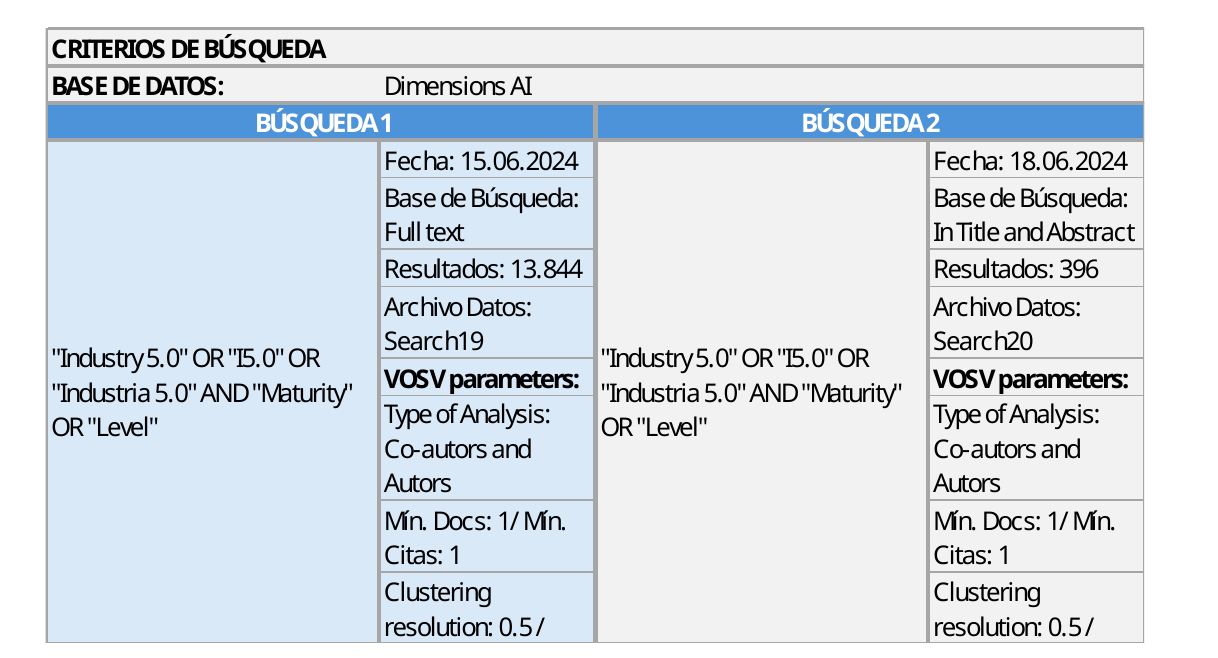
\includegraphics{images/clipboard-3901526380.png}

En la misma tabla se presentan los parámetros base aplicados en VOS
Viewer, resultados que serán presentados más adelante. Como complemento
a las búsquedas en Dimensions AI, se realizó una búsqueda complementaria
en la plataforma abierta Google Scholar, pero dirigida especialmente a
la captura de publicaciones relacionadas directamente con modelos de
madurez de la I5.0. Para tal efecto, la función ``query'' utilizada y
sin restricciones, fue la siguiente: ``industry 5.0 maturity model''.

\subsection{Fase 2: Búsqueda sistemática de la
literatura.}\label{fase-2-buxfasqueda-sistemuxe1tica-de-la-literatura.}

Etapa III: Revisión de la literatura. Tal como se ha señalado, la
revisión de la literatura se realizó fundamentalmente haciendo uso de la
plataforma abierta Dimensions AI con apoyo de Google Scholar,
especialmente para la captura de artículos de interés. Sin perjuicio de
lo anterior, es importante señalar que dada la reciente irrupción del
concepto de Industria 5.0. los artículos, desde el punto de vista del
año de publicación, son en general de mucha actualidad. El Gráfico 1, el
cual está basado en los datos de la ``Búsqueda 1'' (Tabla 2), es decir
la totalidad de las publicaciones encontradas en Dimensions AI, para un
filtro ``Full text'', muestra la temporalidad de los artículos que de
alguna manera vinculan el concepto de la I5.0 y que claramente se
centran en los 2020s.

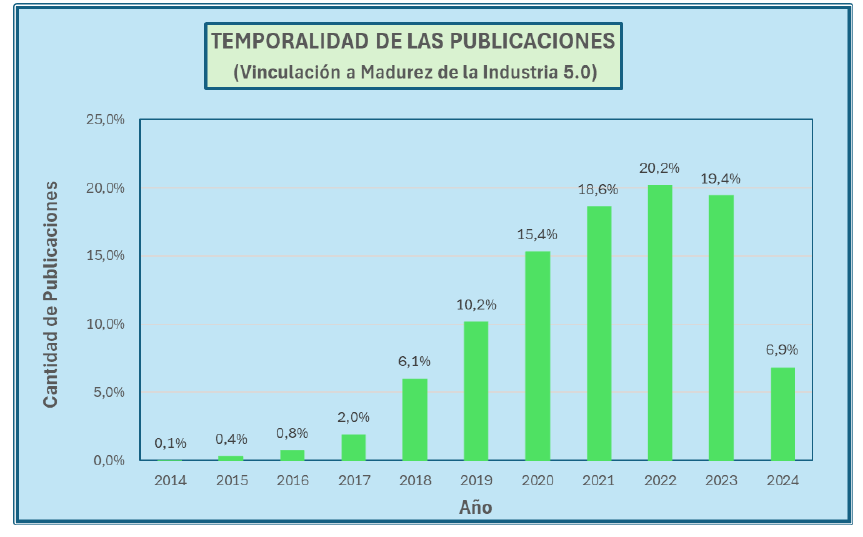
\includegraphics{images/clipboard-1073881894.png}

En términos generales la revisión permitió la selección de artículos,
previo a un análisis de datos mediante la herramienta bibliométrica VOS
Viewer, tomando en consideración las parametrizaciones que se muestran
en la Tabla 2, particularmente el conjunto de publicaciones capturadas
en la ``Búsqueda 2'' y cuyos resultados se presentan a continuación:

\subsubsection{Representación 1: Países de
publicación}\label{representaciuxf3n-1-pauxedses-de-publicaciuxf3n}

Visualización de redes

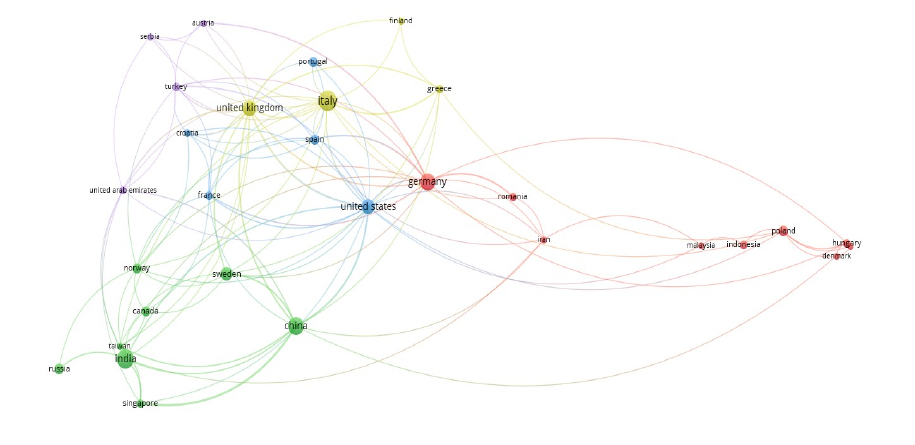
\includegraphics{images/clipboard-216749494.png}

Visualización de superposición:

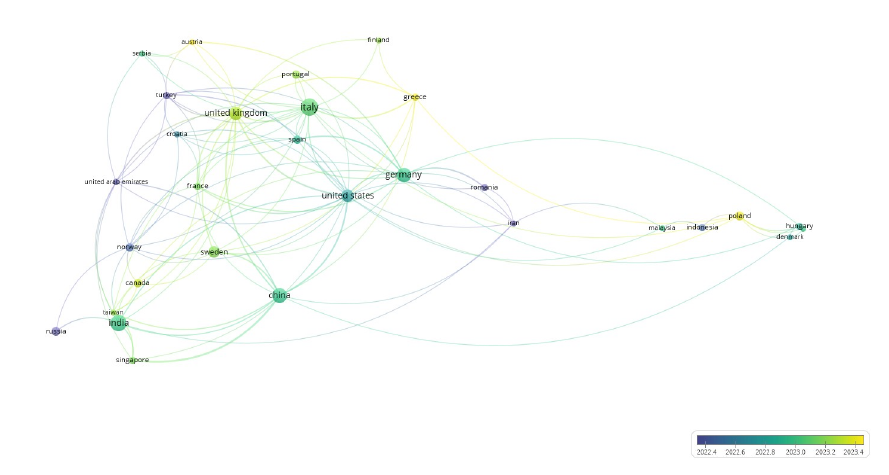
\includegraphics{images/clipboard-3689379518.png}

Visualización de densidad:

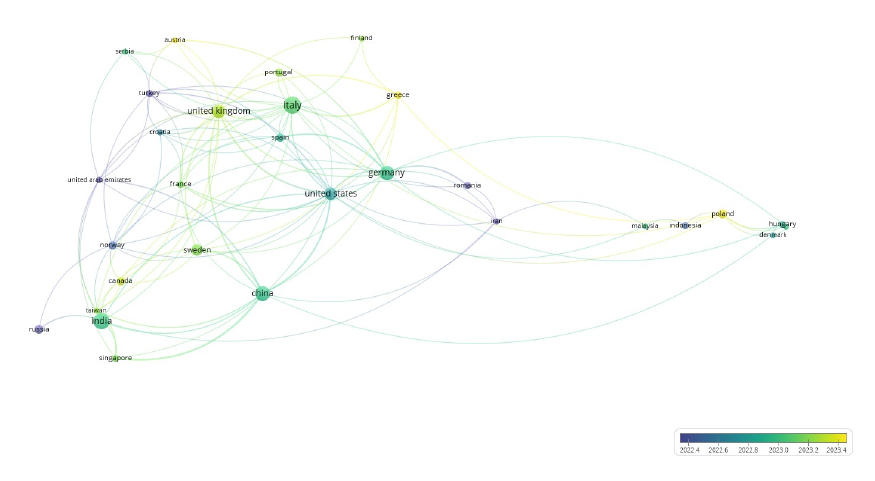
\includegraphics{images/clipboard-3221714897.png}

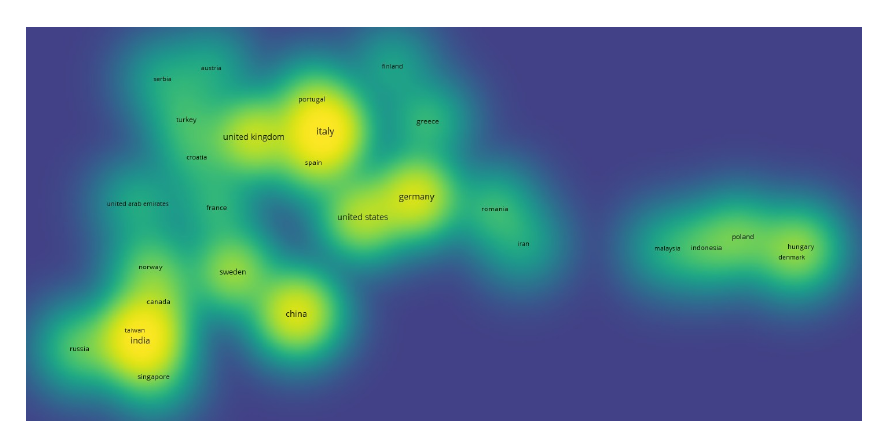
\includegraphics{images/clipboard-3556468416.png}

Desde el punto de vista de los países relacionados con la literatura
rescatada Fig. 3, 4 y 5), se observa claramente una tendencia hacia tres
``clusters'' relevantes como son el de Alemania -- Estados Unidos, el de
Italia -- Portugal -- España -- Reino Unido, el de India -- Canadá y el
de China por si solo, todos los cuales tienen altos grados de
vinculación en redes y claramente una tendencia de temporalidad de las
publicaciones hacia los años más recientes.

\subsubsection{Representación 2: Autores y
Co-Autores}\label{representaciuxf3n-2-autores-y-co-autores}

Visualización de redes:

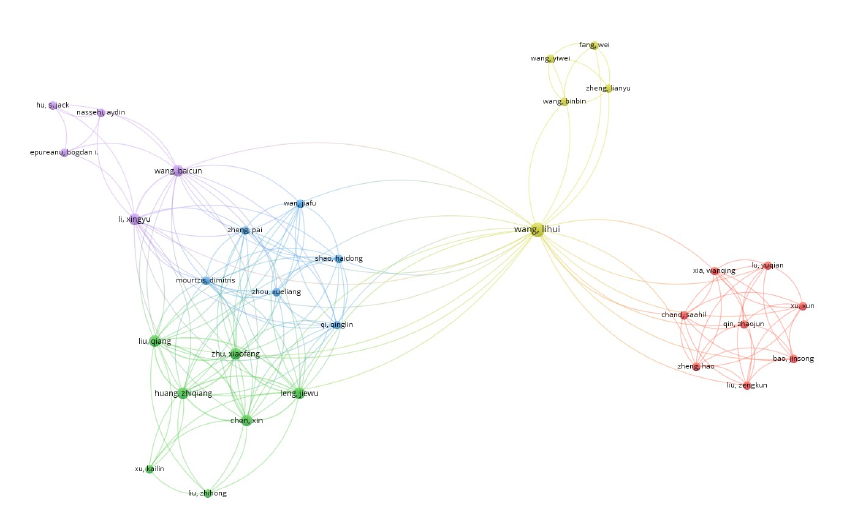
\includegraphics{images/clipboard-148888774.png}

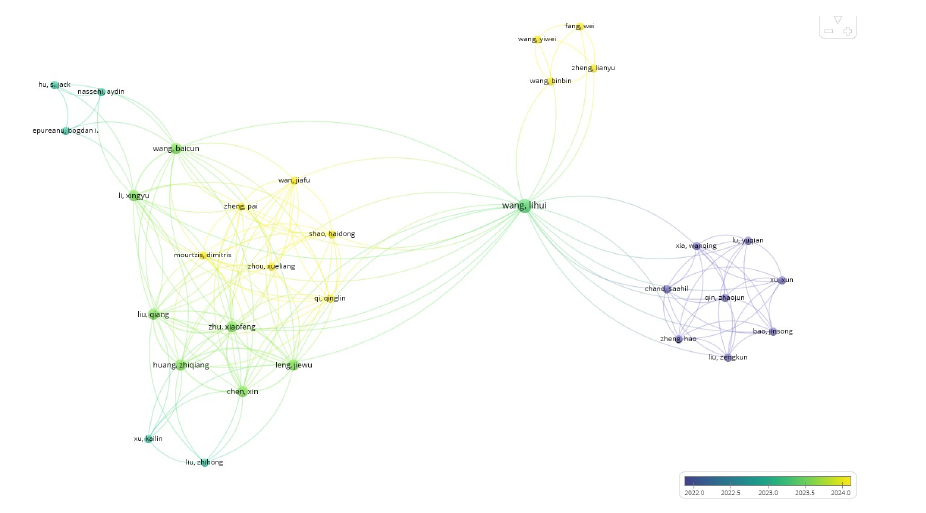
\includegraphics{images/clipboard-1435620609.png}

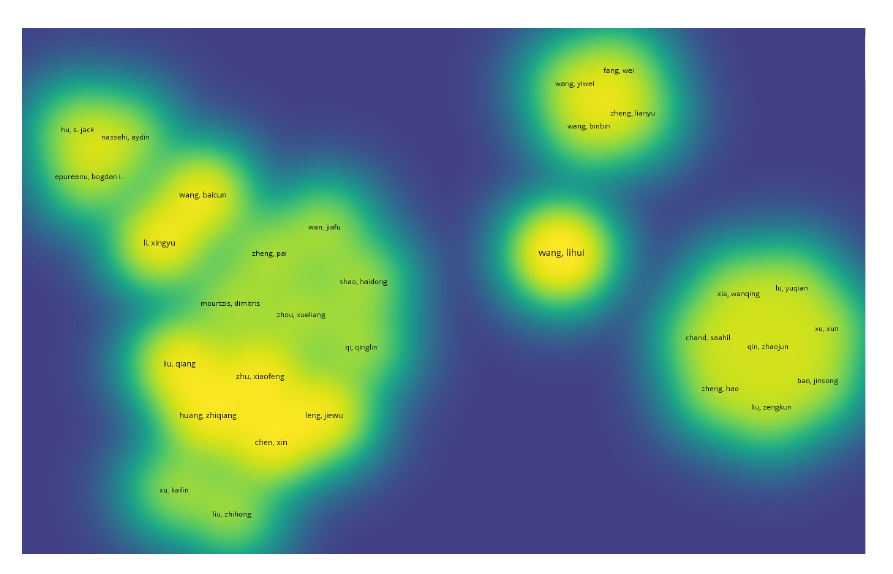
\includegraphics{images/clipboard-2221449078.png}

Desde el punto de vista de los autores, estos se vinculan principalmente
a los países señalados anteriormente, sin embargo, dado que el análisis
se efectuó sobre la masa general de publicaciones que hacen mención a la
I5.0, no hubo una estrecha coincidencia con los autores de las
publicaciones sobre MMs que fueron analizadas, más aún si consideramos
la escasez de artículos que presentan modelos de madurez para la I5.0 o
que de alguna manera se relacionan con ellos. Sin embargo, el catastro
final de publicaciones de análisis, si bien restringido, servirá para
reconocer su vinculación con los distintos temas de interés relacionados
y que pueden servir de base a investigaciones futuras de la I5.0.

\subsubsection{Etapa IV: Filtrado y
categorización.}\label{etapa-iv-filtrado-y-categorizaciuxf3n.}

Siguiendo las bases de las restricciones indicadas por Große-Schwiep et
al., 2020, y señaladas en la Tabla 1, fue posible construir la base de
artículos de análisis, la cual se muestra en la Fig. 9:

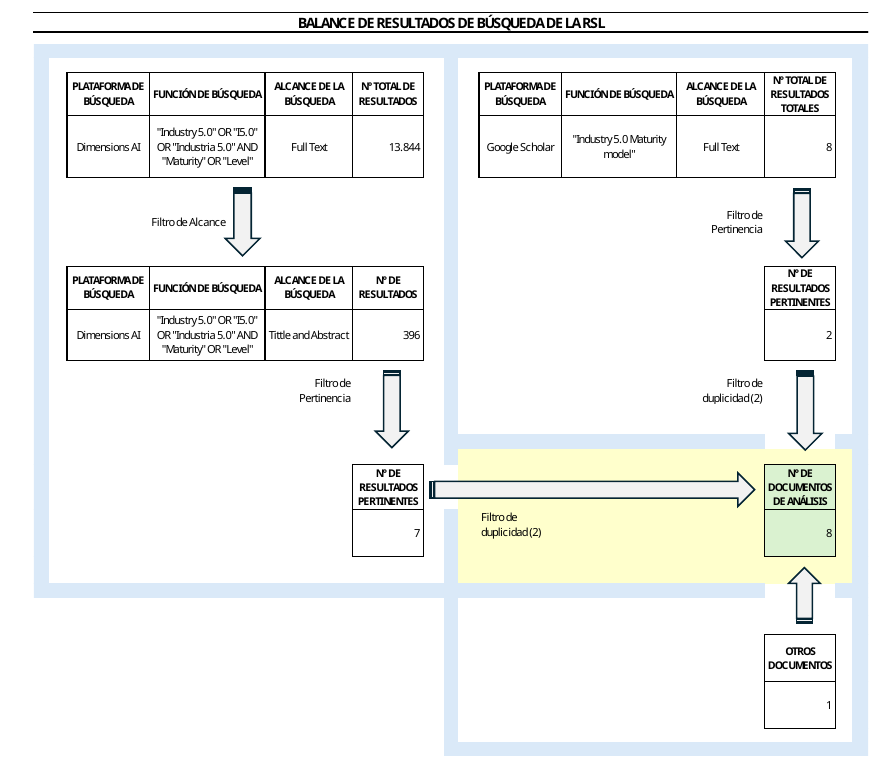
\includegraphics{images/clipboard-2426858467.png}

Los resultados de la Fig. 9, que tomaron como base los resultados
expuestos en la Tabla 1, fueron construidos considerando una base
general de 13.844 documentos seleccionados mediante Dimensions AI y sin
filtros mayores a los establecidos y dentro de cuyo texto (full text) se
encontraron las ``Key words'' incorporadas en la ``query'' respectivas,
selección que se redujo a 396 cuando la búsqueda se circunscribió a los
títulos y abstract de las publicaciones, de las cuales sólo 7 fueron
pertinentes y relevantes para el análisis. Paralelamente, pero sobre la
base de una ``query'' más restrictiva, se realizó una búsqueda en Google
Scholar, la cual arrojó un resultado de sólo 8 publicaciones vinculadas,
las que producto de una revisión general permitió seleccionar sólo 2
artículos pertinentes y relevantes.

Considerando la duplicidad de artículos, la base general de análisis se
redujo a un total de 7 publicaciones, la cual se amplió a 8, con la
incorporación de un artículo adicional del autor.

\subsection{Fase 3: Análisis y
evaluación}\label{fase-3-anuxe1lisis-y-evaluaciuxf3n}

\subsubsection{Etapa V: Análisis y
evaluación}\label{etapa-v-anuxe1lisis-y-evaluaciuxf3n}

En esta etapa se presentan los resultados obtenidos de la RSL, los que
como ya se ha mencionado, corresponden a la revisión y análisis de 8
publicaciones relevantes vinculadas a MMs de la I5.0. Los resultados
obtenidos se presentan en la Tabla 3, la que muestra una caracterización
estructural de los MMs analizados, principalmente respecto de las
dimensiones, factores, criterios y niveles de evaluación. La Tabla 4 por
otra parte, presenta información de cada uno de los MMs de análisis, la
cual está estructurada para entregar las características descriptivas
relevantes de dichos MMs y particularmente sobre la industria de
aplicación, el propósito y alcance del modelo, la o las tecnologías
habilitadoras en las cuales se centra, la cobertura de uno o más de los
pilares de la I5.0 (Centralidad en el humano, resiliencia y
sustentabilidad), el método utilizado en la captura de la información, y
respecto del modelo en sí, la cantidad de dimensiones y/o factores de
construcción, los criterios para la evaluación del estado de madurez y
los niveles propuestos para la clasificación de dicho estado, elemento
fundamental para determinar el punto de partida de la industria respecto
a la industrialización 5.0, pero especialmente para sentar las bases de
una estrategia de desarrollo potencial hacia el posicionamiento de
estadios superiores.

\subsubsection{Modelos de Madurez en Industria
5.0}\label{modelos-de-madurez-en-industria-5.0}

\begin{longtable}[]{@{}
  >{\raggedright\arraybackslash}p{(\columnwidth - 2\tabcolsep) * \real{0.5139}}
  >{\raggedright\arraybackslash}p{(\columnwidth - 2\tabcolsep) * \real{0.4861}}@{}}
\toprule\noalign{}
\begin{minipage}[b]{\linewidth}\raggedright
\textbf{Autores, Año}
\end{minipage} & \begin{minipage}[b]{\linewidth}\raggedright
\textbf{Descripción}
\end{minipage} \\
\midrule\noalign{}
\endhead
\bottomrule\noalign{}
\endlastfoot
\textbf{Arta et al., 2024} & Dimensiones (3) basadas en los 3 pilares de
la I5.0. \textbf{Criterios de Evaluación (11)}: - \textbf{Diseño
centrado en el humano (4)}: Motor innovador, enfoque en empleados,
adaptación holística, requisito para madurez en IA. -
\textbf{Resiliencia (3)}: Política de estabilización, competitividad,
uso de tecnologías modernas. - \textbf{Sostenibilidad (4)}: Soluciones
ambientales, modelo de negocio sostenible, planificación estratégica,
monitoreo. \textbf{Niveles de Madurez (4)}: 0 a 3 (0 = Falta total, 3 =
Alta preparación). \textbf{Base de Evaluación}: Escala Likert (1=No
implementado, 4=Completamente implementado). \\
\textbf{Bajic et al., 2023} & Dimensiones = 3 pilares de la I5.0.
\textbf{Soluciones de soporte (2)}: Tecnológicas y gerenciales. -
Resiliencia: Computación en borde, gemelos digitales, ciberseguridad. -
Sostenibilidad: IA, Big Data, IoT, TQM, WCM. - Centralidad en el humano:
Cobots, colaboración academia-industria. \textbf{Criterios (4)}:
Tecnologías avanzadas, analítica de datos, mejora continua, conocimiento
experto. \textbf{Niveles de madurez (4)}: 1 = Bajo, 4 = Óptimo. \\
\textbf{González-Pérez et al., 2023} & \textbf{Dimensiones (7)}:
Infraestructura tecnológica, métodos de aprendizaje, competencias,
organización, participación ciudadana, innovación social y
sostenibilidad, colaboración y redes. \textbf{Criterios (7)}:
Correspondientes a dimensiones. \textbf{Niveles de madurez (5)}:
Inicial, en Desarrollo, Avanzado, Excelencia, Transformacional. \\
\textbf{Hein-Pensel et al., 2023} & \textbf{Dimensiones (8)}: Diseño
centrado en el humano, resiliencia, sostenibilidad, confiabilidad,
integración tecnológica, alineación estratégica, optimización de
procesos, preparación cultural. \textbf{Criterios (14)} agrupados en 7
categorías (2 por dimensión): Evaluación humana, sostenibilidad,
resiliencia, digitalización, estrategia, colaboración, resultados.
\textbf{Niveles de madurez (4)}: Inicial, Intermedio, Avanzado,
Óptimo. \\
\textbf{Hetmanczyk, 2024} & \textbf{Dimensiones (6)}: Automatización,
robotización, digitalización logística, flexibilidad, intralogística,
integración de sistemas. \textbf{Criterios (3)}: Maquinaria, RR.HH.,
procesos. \textbf{Niveles de madurez (5)}: ML1 (Caótico), ML2
(Definido), ML3 (Planificado), ML4 (Gestionado), ML5 (Optimizado). \\
\textbf{Madhavan et al., 2024} & \textbf{Dimensiones (7)}: Línea de
producción, fuente de energía, procesamiento de mariscos, embalaje,
etiquetado, métodos de prueba y análisis de calidad, proceso empresarial
y comunicación. \textbf{Criterios de Evaluación (7)}: - Enfoque
Humanocéntrico - Sostenibilidad - Resiliencia - Prácticas de Comercio
Justo - Gestión Lean - Documentación y Comunicación - Adopción de
Tecnologías Avanzadas (IoT, IA, nube). \textbf{Niveles de Madurez (6)}:
0 = \emph{Outsider}, 1 = \emph{Beginner}, 2 = \emph{Intermediate}, 3 =
\emph{Experienced}, 4 = \emph{Expert}, 5 = \emph{Leading Performer}. \\
\textbf{Slavic et al., 2024} & \textbf{Dimensiones (3)}:
Human-centricity, sostenibilidad, resiliencia. \textbf{Criterios de
Evaluación (29)}: - \emph{Human-Centricity (10)}: Interfaces, tiempo
real, integración de tareas, innovación, bonificación, capacitación
(específica, multifuncional, digital), seguridad de datos, creatividad.
- \emph{Sostenibilidad (10)}: Gestión ambiental y energética
certificada, eficiencia en materiales, agua, energía, reciclaje,
recuperación, modernización, economía circular. - \emph{Resiliencia
(9)}: Conectividad en tiempo real, instrucciones estandarizadas, robots
móviles y colaborativos, seguridad de datos, software y hardware
específicos, medidas organizacionales, modernización de productos.
\textbf{Niveles de Madurez}: No definidos (modelo no propuesto, pero con
indicadores clave para futuros modelos no binarios). \\
\textbf{Tomassen y Henriksen, 2023} & \textbf{Dimensión (1)}:
Resiliencia. \textbf{Factores de análisis (3)}: Vulnerabilidades,
Capacidades, Tecnología. \textbf{Criterios de Evaluación (27)}: -
\emph{Vulnerabilidades (7)}: Turbulencias, amenazas, presiones externas,
límites de recursos, sensibilidad, conectividad, interrupciones. -
\emph{Capacidades (15)}: Flexibilidad insumos/pedidos, capacidad
productiva, eficiencia, visibilidad, adaptabilidad, anticipación,
recuperación, colaboración, organización, posición en mercado,
seguridad, fortaleza financiera, operadores humanos. - \emph{Riesgos
Globales (5)}: Económicos, Ambientales, Geopolíticos, Sociales,
Tecnológicos. - \emph{Tecnologías habilitadoras}: Todas las digitales
(IA, IoT, fabricación aditiva, etc.). \textbf{Niveles de Madurez}: No
propuestos. \\
\end{longtable}

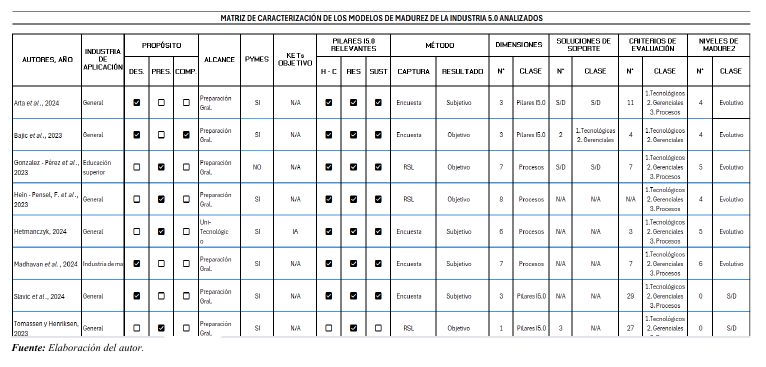
\includegraphics{images/clipboard-275032378.png}

Tal como se muestra en la Tabla 4, los MMs analizados fueron
desarrollados principalmente sin restricciones a la industria de
aplicación (General), lo cual permitiría su aplicación a la industria en
general. Sin embargo, dos de los modelos presentados, fueron
desarrollados en relación directa con industrias específicas, como el
propuesto por González-Pérez et al., 2023, el cual está enfocado en las
instituciones de educación superior y el de Madhavan et al., 2024
centrado en la Industria de mariscos. Desde el punto de vista del
propósito u objetivo de los MMs, se puede observar que en general estos
fueron concebidos con dos propósitos, uno, el ``Descriptivo'', es decir,
para determinar el estado de madurez actual de una empresa y otro, el
``Prescriptivo'', los que tienen como objetivo proveer un modelo
normativo con recomendaciones para actuar en línea con el logro de una
estrategia de proyección hacia estados de madurez superiores. Sin
embargo, ninguno de ellos fue del tipo ``Comparativo'', es decir,
concebidos para entregar directrices hacia la evaluación de empresas en
términos comparativos en el ámbito tanto interno como externo a la
organización. Otra de las características relevantes de los MM de
análisis, fue la determinación del alcance funcional a la
industrialización 5.0, es decir, su caracterización respecto de si ellos
fueron definidos para evaluar el nivel de madurez desde la perspectiva
de la preparación general a la implementación de la I5.0 (Ej. a nivel de
la cadena de suministro global) o con una visión unitecnológica, es
decir, desde la óptica de la preparación a la I5.0, pero en relación a
una o varias de las tecnologías habilitantes de la Industria 4.0 (KETs),
como por ejemplo, inteligencia artificial (IA), analítica de grandes
datos (BDA), Internet de las cosas (IoT), ciber seguridad, entre otras.
Los resultados de los MM revisados muestran que en general ellos fueron
desarrollados para evaluar el status de la industria respecto de la
preparación integral a la implementación de la I5.0 y sólo uno de ellos
es de carácter unitecnológico, el que particularmente se centra en la
determinación del nivel de madurez para la preparación a la IA. Desde la
perspectiva de los pilares de la I5.0, los modelos de madurez pueden
estar concebidos, estructurados o centrados tomando en consideración uno
o más de estos pilares o dimensiones fundamentales. En tal sentido,
siete de los ocho modelos de madurez analizados toman en consideración
los tres pilares de la I5.0 (Centralidad en el humano, Resiliencia y
Sustentabilidad) y sólo uno de ellos se centró en uno de los pilares,
particularmente la resiliencia. Dada la importancia que las PyMEs tienen
en las economías de los países y ciertamente las restricciones y
limitaciones que enfrentan a los procesos de innovación y/o de adopción
tecnológica, fue importante conocer de los modelos analizados, la
adaptación u orientación que ellos tienen respecto de la evaluación de
los niveles de madurez de la Industria 5.0, pero específicamente en el
contexto de las PyMEs. En tal sentido, la casi totalidad de los MM
consideran como relevante su aplicación a las PyMEs y sólo uno de ellos,
el de González -- Pérez et al., 2023, no lo menciona dentro de sus
objetivos, pero tampoco menciona que ha sido preparado para grandes
compañías. La singularidad de este modelo radica en que está
estructurado para la determinación del estado de madurez en
instituciones de educación superior, las que en general no están
insertas dentro del segmento empresarial de las PyMEs. Por último, y
como una forma de caracterizar los MM respecto a la base de captura de
la información y el tipo de resultados obtenidos, se preparó una base
que considera 4 opciones para la captura de la información de soporte:
Encuesta, RSL, Intervención en la empresa y un método mixto. En base a
estos métodos de captura, los resultados que se obtienen son subjetivos
al tratarse de encuestas, objetivos en base a RSLs e intervención y
mixto para procesos mixtos de captura. En el caso de este estudio, los
MMs analizados responden a una captura de datos en base a encuestas y
RSLs, no encontrándose hasta ahora MMs en dónde la captura haya sido
producto de un trabajo interno y directo en las empresas. Ahora bien, si
hacemos un análisis más en profundidad de los modelos analizados, es
decir desde la perspectiva de su estructura, podemos ver que el
denominador común es la propuesta de un modelo para determinar el estado
de preparación a la implementación de la I5.0, pero de alguna manera
tomando en consideración las tecnologías de la I4.0, lo que implica la
digitalización integral de la empresa, pero asumiendo el rol relevante
que deben tener los pilares de la I5.0 en ese proceso. La implementación
de tecnologías avanzadas o inteligentes no pueden abstraerse de las
dimensiones estructurales de la I5.0 como son la centralidad en la
gestión desde la perspectiva humana, la resiliencia para adaptarse a los
cambios del entorno y recuperar los niveles iniciales a eventos
disruptivos, los que pueden gatillar transformaciones de la empresa y
sus modelos de negocios, sin descuidar los principios de la
sustentabilidad, todos ejes esenciales para garantizar la competitividad
de las compañías y la continuidad del negocio. Para la realización de un
análisis de los MMs seleccionados, desde la perspectiva de sus
dimensiones, debemos complementar con los resúmenes descriptivos que se
muestran en la Tabla 3. De ellos se desprende que en general los MM
definen sus dimensiones de base, ya sea en una relación directa con los
Pilares de la I5.0 o desde la mirada de los procesos propios de la
industria, pero enfocados igualmente en esos mismos pilares y, por ende,
la cantidad de dimensiones va de 3 y más, respectivamente. Si entramos a
revisar más en profundidad los MM, esta vez ya enfocándose en los
criterios de evaluación, es decir, las interrogantes de base para
determinar el estadio de la empresa respecto del objetivo central de
cada MM, la situación se hace algo más compleja, ya que existen puntos
de divergencia estructural importantes en su formulación. Sin embargo, a
pesar de esta divergencia, se pudo constatar que de alguna manera todos
ellos definen sus criterios sobre la base de tres elementos relevantes:

a)- Criterios tecnológicos: Basados en la situación tecnológica de la
empresa como elemento determinante de la madurez.

b)- Criterios Gerenciales: Basados en factores de análisis gerencial al
interior de la empresa, ya sea en términos de sus estrategias y/o
modelos de negocio, como de las políticas internas en distintas áreas,
por ejemplo, en gestión de recursos humanos al tratarse del pilar humano
-- céntrico de la I5.0, o de la aplicación de modelos de excelencia
operacional (gestión Lean, metodologías Agiles, TPM, entre otras.

c)- Criterios de Procesos: Centrados en la gestión de procesos propios
de la naturaleza de la empresa o bien con un alcance general adecuado a
toda industria.

Dentro de los MM analizados, como ya se ha señalado, no hay convergencia
en términos de la estructura y el foco central de ellos.

Un ejemplo de ello es el MM propuesto por Madhavan et al., 2024, el cual
considera una estructura basada en siete criterios de evaluación. Un
criterio central Humano- céntrico para evaluar la adopción de prácticas
de gestión que prioricen el bienestar de los empleados y la interacción
humano-máquina; otro respecto a la sostenibilidad para ver de qué manera
la empresa asume prácticas sostenibles que reduzcan los impactos
económicos, ambientales y sociales negativos; un tercero enfocado en la
resiliencia, para evaluar la existencia y efectividad de planes para
manejar interrupciones económicas y ambientales; un cuarto que considera
en nivel de adopción de ``Prácticas de Comercio Justo'' que promuevan la
transparencia y la trazabilidad a lo largo de la cadena de valor; otro
para evaluar la aplicación de metodologías de Gestión Lean, midiendo de
que forma la organización implementa acciones para la reducción de
desperdicios y la gestión eficiente de recursos; un criterio basado en
los procesos de Documentación y Comunicación, incluyendo el uso de
sistemas integrados y análisis de datos y finalmente, un criterio para
medir el nivel de ``Adopción de Tecnologías Avanzadas'' como IoT,
inteligencia artificial y cloud computing, como una forma de mejorar la
apertura empresarial y la orientación al mercado. Claramente el MM de
Madhavan et al., 2024, responde a una estructura centrada en los tres
pilares de la I5.0, pero con criterios de evaluación divergente de otros
modelos cuyos objetivos son ciertamente distintos. Por otra parte, si
observamos el MM de Hetmanczyk, 2024, el cual es de carácter
unitecnológico y basado directamente en la evaluación de la industria
respecto a su estado de preparación para la implementación de
tecnologías de inteligencia artificial, son seis las dimensiones que
propone, las cuales se evalúan respecto de tres criterios como:
Maquinaria, infraestructura y equipos; Recursos humanos y Procesos, los
cuales se evalúan desde la base de una estructura de seis dimensiones
como son la Automatización de procesos de producción, Robotización de
procesos de producción, Digitalización de procesos de intralogística en
almacenes (optimización de inventario); Flexibilidad de los sistemas de
producción (capacidad de respuesta a cambios en el mercado); 5.
Intralogística de procesos de producción (Automatización ágil en flujos
de materiales y productos) e Integración de sistemas de gestión.
Finalmente, y en lo que si ha sido posible encontrar coincidencia entre
los MMs, es en lo que respecta a los niveles de madurez, ya que todos
ellos y como es propio en general de los MMs, cualquiera sea el objetivo
que tengan, se estructuran sobre la base de niveles de madurez
``evolutivos'', es decir en una escala de evaluación que va desde un
nivel inicial o básico respecto de un criterio en particular, hasta
estadios evolutivos superiores de máxima preparación, adecuación,
relevancia, etc., respecto al criterio analizado, en una escala que
ciertamente es diversa según los criterios definidos por cada autor.
Ejemplos de estas diferencias se presentan al comparar la propuesta de
Hein-Pensel, F. et al., 2023, que propuso un MM basado en 4 niveles de
madurez (NM) respecto a la digitalización vinculada a los pilares de la
I5.0, desde un estadio Inicial de baja digitalización y falta de
estrategias para la implementación de tecnologías avanzadas, hasta un
nivel Óptimo de digitalización completa y con enfoque en la
sostenibilidad y la resiliencia y utilización de la IA centrada en el
ser humano para mejorar la toma de decisiones y la eficiencia operativa.
Pasando por un estado Intermedio con iniciación en la implementación de
algunas tecnologías digitales, pero limitada integración y uso efectivo
y un estado Avanzado con utilización de tecnologías digitales de manera
efectiva e inicio de la integración de la IA en sus procesos. El proceso
de revisión y análisis de los MM considerados permitió observar las
divergencias estructurales entre ellos y evidenciar la dificultad de
homologación en términos de su estructura, ya que claramente su
concepción está directamente condicionada por los objetivos que
persiguen, lo cual condiciona la definición de sus dimensiones y
criterios de evaluación.

\section{Conclusiones y
recomendaciones}\label{conclusiones-y-recomendaciones}

Sobre la base de la revisión y análisis de los MM expuestos, ha sido
posible extraer algunas conclusiones y recomendaciones que permiten
delinear trabajos futuros sobre el tema y particularmente de las
consideraciones relevantes orientadas a la formulación de MM integrados
entre las Industrias 5.0 y 4.0. Si bien el concepto de la I5.0, a pesar
de su irrupción reciente en la gestión industrial, se manifiesta en una
nutrida literatura y en diferentes latitudes, pero poca evidencia fue
encontrada respecto de la existencia de MMs propios de la I5.0. Sin
perjuicio de lo anterior, el trabajo logró identificar algunos
documentos que presentan tanto MM específicos de la I5.0 como otros que
entregan bases y conceptos generales para su formulación, todos los
cuales de alguna manera permiten conocer las bases estructurales de su
concepción y la forma en que ellos se vinculan con la I4.0. Del estudio
se desprende que en todos los MM analizados existe un denominador común
en la propuesta de un modelo para determinar el estado de preparación a
la implementación de la I5.0, pero sobre una base habilitante de las
tecnologías 4.0, lo que lleva a develar el vínculo funcional entre ambas
industrias desde la perspectiva de la digitalización al servicio de los
pilares de la I5.0 y por lo tanto, no siendo posible la concepción de un
modelo, sin considerar los aspectos tecnológicos, pero desde una mirada
humano céntrica para centrarse en objetivos sociales, de resiliencia
para adaptarse a los cambios del entorno ante eventos disruptivos, los
cuales pueden llevar incluso a transformaciones profundas de la empresa
y sus modelos de negocio, y de la sustentabilidad en toda la cadena de
valor, todas bases fundamentales para garantizar la competitividad de
las compañías y su permanencia en el mercado. En detalle han sido
expuestas en el capítulo anterior, las principales diferencias entre los
modelos analizados, los cuales son ciertamente el reflejo de sus
objetivos específicos, diferencias que de alguna manera tienen especial
relevancia a la hora de trabajar en la formulación de un MM integrado
entre las I5.0 e I4.0 y que son relevantes a la hora de definir los
objetivos particulares que de ellos se espera. Resulta importante
resaltar que la totalidad de los MMs presentados fueron concebidos en
base, tanto a propósitos descriptivos como prescriptivos, lo que lleva a
concluir que un objetivo relevante de ellos y ciertamente relevante para
la industria, es la presentación de resultados respecto del nivel de
madurez de las empresas con énfasis en bases estructurales tecnológicas,
gerenciales y/o de procesos, ya que desde allí será posible construir
pilares para la definición de estrategias que permitan alcanzar niveles
o estadios superiores de desarrollo potencial, sobre la base de una
escala de valoración que va desde niveles básicos o incipientes de
habilitación o desarrollo hasta niveles avanzados u óptimos desde la
mirada de las dimensiones y criterios de evaluación particulares que
presentan tales MMs. Independiente del propósito de los modelos
analizados, parece fundamental definir qué es lo que el MM pretende
medir, y en tal sentido, la mayoría de ellos se estructura sobre la base
de la medición del nivel de madurez en la perspectiva de determinar el
grado de preparación general en que las organizaciones se encuentran
respecto la I5.0, tomando en consideración sus tres pilares
fundamentales como son la centralidad en el ser humano, la resiliencia y
la sustentabilidad, asumiendo el rol fundamental que ejercen las
tecnologías 4.0, es decir la aplicación de tecnologías no sólo con un
objetivo basado en la rentabilidad del negocio, sino con una estrecha
vinculación con los paradigmas propios de la I5.0. Este camino lógico y
coherente con la evolución natural de las empresas ante cualquier
proceso transformador a que la industria las enfrente, no puede estar
ajeno a las limitaciones y/o restricciones propias vinculadas a su
gestión y las influencias del entorno en el cual se desenvuelven,
efectos que son más determinantes al tratarse de empresas PyMEs, las que
por su tamaño y condicionantes, principalmente relacionadas con el
acceso al capital, se enfrentan a procesos de adopción tecnológica
retardados y que por ende, las estrategias que en esta materia se
determinen para este segmento empresarial, en ningún caso podrán dejar
de considerar la realidad que enfrentan, cuestión que los MMs que se
formulen deberán tener presente como elemento central. Finalmente, y a
la luz de los resultados y conclusiones obtenidos y especialmente de la
escasez de modelos de madurez encontrados hasta ahora, parece
interesante ampliar y profundizar dicha búsqueda hacia modelos de
madurez de la Industria 4.0 con posterioridad al año 2020 para medir el
grado de influencia que en sus definiciones de base tienen los pilares
de la I5.0 y de qué manera ellos están abordando estos valores
fundamentales de la transformación de la industria. En tal sentido,
aspectos como los efectos sobre el trabajo y las compensaciones
pecuniarias y no pecuniarias a los empleados, los aspectos culturales de
las organizaciones y los efectos sobre la eficiencia en su gestión, la
capacidad con que las empresas se preparan ante la ocurrencia de eventos
disruptivos capaces de transformar los modelos negocio de éstas y los
efectos de la sustentabilidad y sus factores inherentes, deben ser
aspectos estructurales relevantes de evaluación, más aún como respuesta
a un mundo industrial influenciado por el cambio climático, la escasez
de recursos y la globalización, entre otros, lo cual debe ser parte de
la estrategia de las compañías para lograr un mayor posicionamiento
competitivo en el mercado e incluso su supervivencia..

\section*{Referencias
bibliográficas}\label{referencias-bibliogruxe1ficas}
\addcontentsline{toc}{section}{Referencias bibliográficas}

\phantomsection\label{refs}
\begin{CSLReferences}{1}{0}
\bibitem[\citeproctext]{ref-arnold2018industry4adoption}
Arnold, Christian, Johannes W. Veile, and Kai-Ingo Voigt. 2018. {``What
Drives Industry 4.0 Adoption? An Examination of Technological,
Organizational, and Environmental Determinants.''}
\url{https://scholar.google.com/scholar?hl=es&as_sdt=0\%2c5&q=what+drives+industry+4.0+adoption\%3f+an+examination+of+technological\%2c+organizational\%2c+and+environmental+determinants&btng=}.

\bibitem[\citeproctext]{ref-arta2024industry5readiness}
Arta, M., N. Mandagi, I. Kurniawan, and E. Abdurachman. 2024.
{``Industry 5.0 Readiness Assessment: A Maturity Models for Indonesian
Companies.''} \emph{Journal Eduvest} 4 (5): 4355--74.
\url{https://eduvest.greenvest.co.id/index.php/edv/article/view/1303}.

\bibitem[\citeproctext]{ref-bajic2023fuzzi5maturity}
Bajic, B., S. Moraca, and A. Rikalovic. 2023. {``Fuzzi Maturity Models
for Smart Manufacturing Readiness: Industry 5.0 Perspective.''}
\url{https://ieeexplore.ieee.org/abstract/document/10174102}.

\bibitem[\citeproctext]{ref-brocke2009giant}
Brocke, J. vom, A. Simons, B. Niehaves, K. Reimer, R. Plattfaut, and A.
Cleven. 2009. {``Reconstructing the Giant: On the Importance of Rigour
in Documenting the Literature Search Process.''} In \emph{ECIS 2009
Proceedings}. Vol. 161.
\url{https://aisel.aisnet.org/cgi/viewcontent.cgi?article=1145&context=ecis2009}.

\bibitem[\citeproctext]{ref-carolis2017maturitymodel}
Carolis, Anna de, Marco Macchi, Elisa Negri, and Sergio Terzi. 2017.
{``A Maturity Model for Assessing the Digital Readiness of Manufacturing
Companies.''} In \emph{IFIP International Conference on Advances in
Production Management Systems (APMS)}, 13--20.
\url{https://hal.inria.fr/hal-01666224/document}.

\bibitem[\citeproctext]{ref-dahl2021sawmill}
Dahl, P. 2021. {``Improving Sawmill Scheduling Through Industry 4.0 -- a
CASE Study at VIDA AB.''} Master's thesis, Swedish University of
Agricultural Sciences, SLU.
\url{https://stud.epsilon.slu.se/17364/3/dahl_p_211106.pdf}.

\end{CSLReferences}

\bibliographystyle{unsrt}
\bibliography{references.bib}


\end{document}
